\documentclass[11pt,letterpaper,boxed]{pset}

\usepackage[margin=0.75in]{geometry}
\usepackage{ulem}

\begin{document}

    \problemlist{PHYS051 HW04}
    \begin{center}
        P28.13, SUP 4A, E30.22, *E30.25, P30.13, P30.24

    \end{center}
    
    \begin{problem} [P28.13]
    On a thin rod of length $L$ lying along the $x$ axis with one end at the origin ($x=0$), as in Fig. 28-46, there is distributed a charge per unit length given by $\lambda=kr$, where $k$ is a constant and $r$ is the distance from the origin. 
    
    \begin{itemize}
        \item [(a)] Taking the electrostatic potential at infinity to be zero, find $V$ at the point $P$ on the $y$ axis. 
        \item [(b)] Determine the vertical component, $E_y$, of the electric field at $P$ from the result of part (a) and also by direct calculation.
        \item [(c)] Why cannot $E_x$, the horizontal component of the electric field at $P$, be found using the result of part (a)?
        \item [(d)] At what distance from the rod along the $y$ axis is the potential equal to one-half the value at the left end of the rod?
    \end{itemize}
    \end{problem}
    \begin{figure*} [ht]
        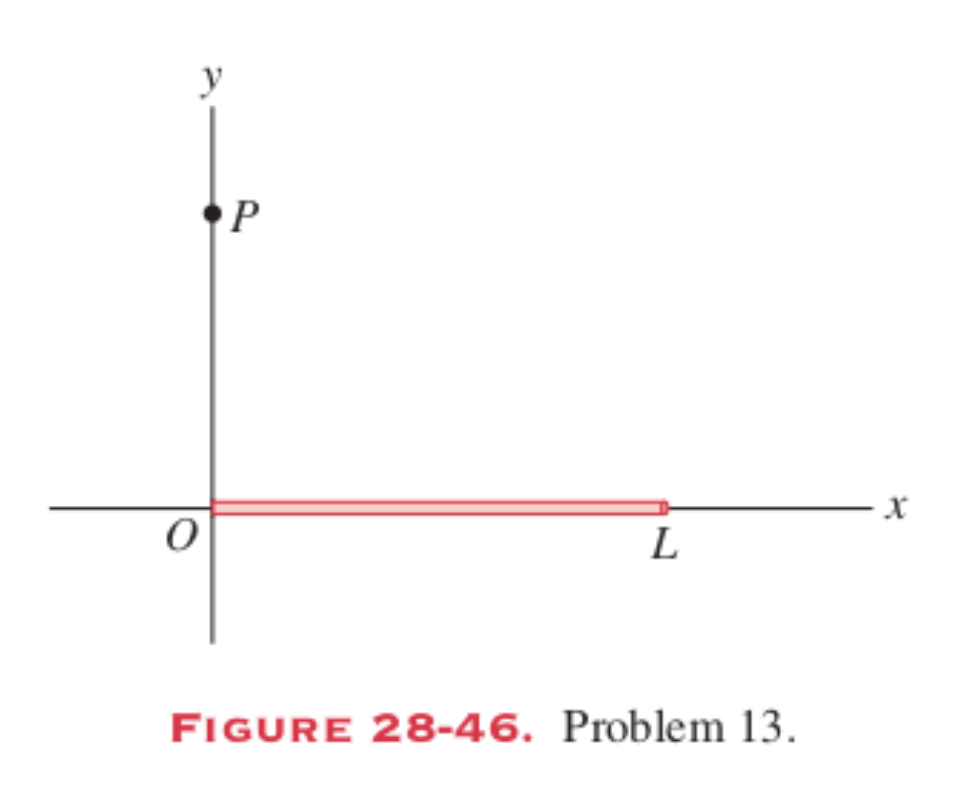
\includegraphics[width=150px]{HW4Images/P28-13.png}
        \label{fig:P28-13}
    \end{figure*}
    \newpage
    
    \begin{problem} [SUP 4A]
    Consider the vector field $\Vec{C}=-y\hat{i}+x\hat{j}$ in the $x$-$y$ plane.
    
    \begin{itemize} 
        \item [(a)] Sketch the field lines.
        \item [(b)] Calculate $\Vec{\nabla} \times \Vec{C}$.
        \item [(c)] Calculate $\oint \Vec{C} \cdot \Vec{dl}$ over the closed curve $x^2+y^2=1$.
        \item [(d)] Show that Stokes' theorem holds by evaluating $\int (\Vec{\nabla} \times \Vec{C}) \cdot \Vec{dA}$ over a surface bounded by the curve in part (c).
    \end{itemize}
    \end{problem}
    \newpage
    
    \begin{problem} [E30.22]
    Attempts to build a controlled thermonuclear fusion reactor, which, if successful, could provide the world with a vast supply of energy from heavy hydrogen in seawater, usually involve huge electric currents for short periods of time in magnetic field windings. These currents are often provided by discharging large banks of capacitors. One such capacitor bank provides 61.0 mF at -10.0 kV. Calculate the stored energy
    
    \begin{itemize}
        \item [(a)] in joules.
        \item [(b)] in kW $\cdot$ hr. Comment on whether this is a large or small number of kW $\cdot$ hr.
    \end{itemize}
    \end{problem}
    \newpage
    
    \begin{problem} [*E30.25]
    An isolated metal sphere whose diameter is 12.6 cm has a potential of 8150 V (where $V=0$ at infinity). Calculate the energy density in the electric field near the surface of the sphere.
    \end{problem}
    \newpage
    
    \begin{problem} [P30.13]
    \begin{itemize}
        \item [(a)] Calculate the energy density of the electric field at a distance $r$ from an electron (presumed to be a particle) at rest.
        \item [(b)] Assume now that the electron is not a point but a sphere of radius $R$ over whose surface the electron charge is uniformly distributed. Determine the energy associated with the external electric field in vacuum of the electron as a function of $R$.
        \item [(c)] If you now associate this energy with the mass of the electron, you can, using $E_0=mc^2$, calculate a value for $R$. Evaluate this radius numerically; it is often called the classical radius of the electron.
    \end{itemize}
    \end{problem}
    \newpage
    
    \begin{problem} [P30.24]
    A dielectric slab of thickness $b$ is inserted between the plates of a parallel-plate capacitor of plate separation $d$. Show that the capacitance is given by
    
    \[C = \frac{\kappa_e\epsilon_0A}{\kappa_ed-b(\kappa_e-1)}\]
    
    (Hint: Derive the formula lfollowing the pattern of Sample Problem 30-9.) Does this formula predict the correct numerical result of the sample problem? Verify that the formula gives reasonable results for the special cases of $b=0$, $\kappa_e=1$, and $b=d$.
    \end{problem}
    \newpage
\end{document}